% % % % % Packages % % % % %
\documentclass[11pt]{scrartcl}
\usepackage[sexy]{evan}
\usepackage{imakeidx}
\usepackage{amsmath}
\usepackage{amssymb}
\usepackage{mathtools}
\makeindex[columns=3, title=Alphabetical Index, intoc]
% \usepackage[left=2cm, right=2cm, top=1cm, bottom=2cm]{geometry}
\usepackage{graphicx}
\newcommand*{\rom}[1]{\expandafter\@slowromancap\romannumeral #1@}
% alert -> blue sent
% vocab -> word
% lstlisting
% \begin{lstlisting}[language=C++,basicstyle=\small\ttfamily], [basicstyle=\scriptsize\ttfamily]
% \linespread{1.25}

\newcommand{\mat}[1]{\begin{bmatrix} #1 \end{bmatrix}}

% % % % % Information % % % % %
\title{Ski Resort Database Design}
\author{Group 14: Connor, Luis, Mohammad, Nathan}
\date{Spring 2025}
\hypersetup
{
  pdfauthor={Group 14},
  pdfsubject={HWs CSC 460},
  pdftitle={CSC 460: Homeworks},
}
\begin{document}
\maketitle
\tableofcontents

\section{Conceptual database design}
Figure~\ref{fig:er_diagram} shows the E--R diagram of the ski resort database. 
To design the conceptual schema of the database we first did a detailed walk through fot the program specifications to record what tables are going to be needed to store data. 
The ER diagram we made captures the ski resorts day to day operations tracking members and their activites as well as the resorts staff and income via its services. Attributes
are constrained via sql datatypes.

\begin{figure}[h]
  \centering
  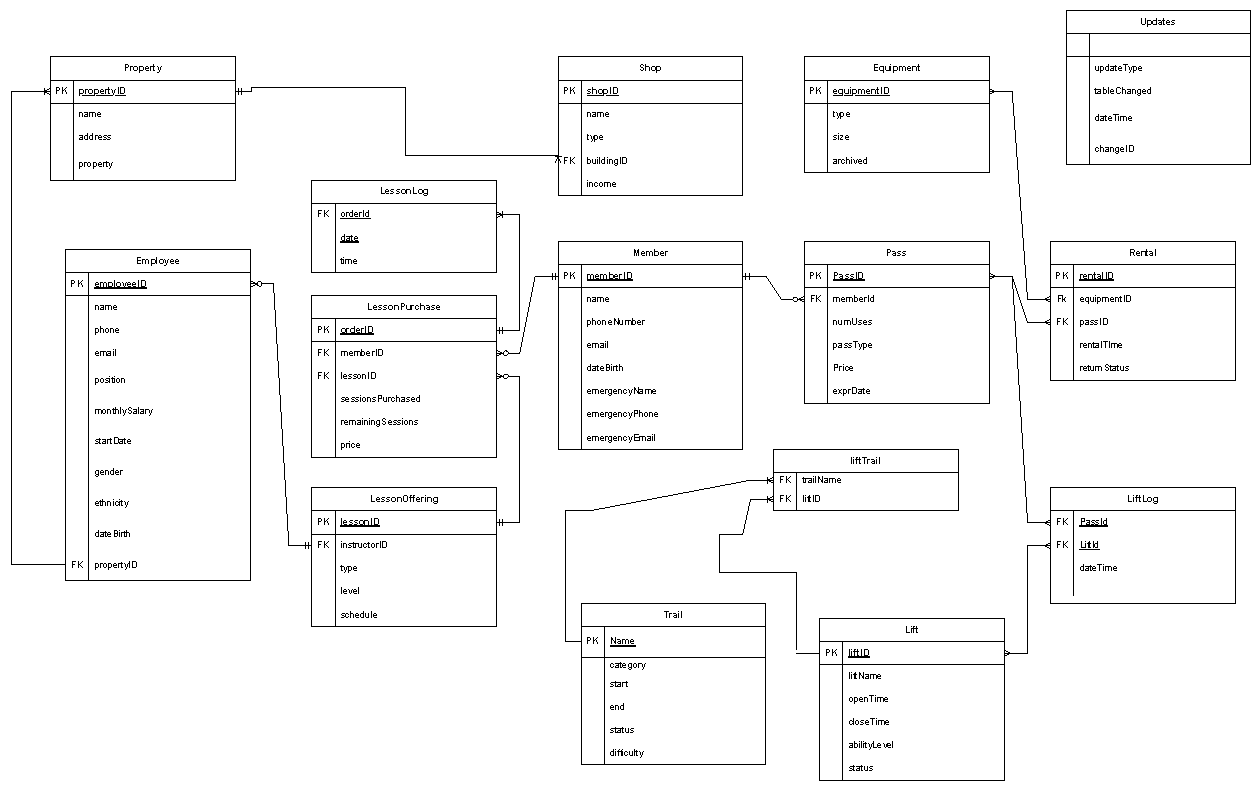
\includegraphics[width=1.1\textwidth]{er.pdf}
  \caption{E--R Diagram of the Ski Resort Database}
  \label{fig:er_diagram}
\end{figure}

\section{Logical database design}

Below is the final relational schema derived from the E--R diagram. Each table lists its attributes, primary keys (\textbf{PK}), and foreign keys (\textbf{FK}) explicitly. 
This design reflects a direct and normalized translation of the conceptual model into the relational model used in Oracle SQL.

\begin{itemize}
  \item \textbf{Property(} \underline{propertyID}, name, address, propertyType \textbf{)}

  \item \textbf{Shop(} \underline{shopID}, name, shopType, buildingID\textsuperscript{FK}, income \textbf{)}

  \item \textbf{Equipment(} \underline{equipmentID}, equipmentType, equipmentSize, archived \textbf{)}

  \item \textbf{Rental(} \underline{rentalID}, equipmentID\textsuperscript{FK}, passID\textsuperscript{FK}, rentalTime, returnStatus \textbf{)}

  \item \textbf{Pass(} \underline{passID}, memberID\textsuperscript{FK}, numUses, passType, price, exprDATE \textbf{)}

  \item \textbf{LiftLog(} passID\textsuperscript{FK}, liftID\textsuperscript{FK}, dateTime \textbf{)}

  \item \textbf{Lift(} \underline{liftID}, liftName, openTime, closeTime, abilityLevel, status \textbf{)}

  \item \textbf{TrailLift(} liftID\textsuperscript{FK}, trailName\textsuperscript{FK} \textbf{)}

  \item \textbf{Trail(} \underline{name}, category, startPos, endPos, status, difficulty \textbf{)}

  \item \textbf{Member(} \underline{memberID}, name, phoneNumber, email, dateBirth, emergencyName, emergencyPhone, emergencyEmail \textbf{)}

  \item \textbf{LessonLog(} orderID\textsuperscript{FK}, dateTime \textbf{)}

  \item \textbf{LessonPurchase(} \underline{orderID}, memberID\textsuperscript{FK}, lessonID\textsuperscript{FK}, sessionsPurchased, remainingSessions, price \textbf{)}

  \item \textbf{LessonOffering(} \underline{lessonID}, instructorID\textsuperscript{FK}, lessonType, skillLevel, schedule \textbf{)}

  \item \textbf{Employee(} \underline{employeeID}, name, phone, email, position, monthlySalary, startDate, gender, ethnicity, dateBirth, propertyID\textsuperscript{FK} \textbf{)}

  \item \textbf{Updates(} updateType, tableChanged, changeID, dateTime \textbf{)}
\end{itemize}

\section{Normalization analysis}
\section*{Normalization Analysis}

All relations in the schema adhere to the First Normal Form (1NF) as all attributes are not set values. 
They also conform to the Second Normal Form (2NF) since all non-prime attributes are fully functionally dependent on the candidate key(s). 
Below, we analyze each relation for Boyce-Codd Normal Form (BCNF) or the Third Normal Form (3NF).

\subsection*{1. \texttt{Property(propertyID, name, address, propertyType)}}
\begin{itemize}[leftmargin=2em]
  \item \textbf{Functional Dependencies:}
    \begin{align*}
      \text{propertyID} &\rightarrow \text{name, address, propertyType}
    \end{align*}
  \item \textbf{Candidate Key:} propertyID
  \item \textbf{BCNF Status:} \textit{Yes}, all functional dependencies have a superkey on the left-hand side.
\end{itemize}

\subsection*{2. \texttt{Shop(shopID, name, type, buildingID, income)}}
\begin{itemize}
  \item \textbf{FDs:} shopID $\rightarrow$ name, type, buildingID, income
  \item \textbf{PK:} shopID
  \item \textbf{BCNF:} Yes because all attributes are functionally dependent on the primary key.
\end{itemize}

\subsection*{3. \texttt{Equipment(equipmentID, type, size, archived)}}
\begin{itemize}
  \item \textbf{FDs:} equipmentID $\rightarrow$ type, size, archived
  \item \textbf{PK:} equipmentID
  \item \textbf{BCNF:} Yes, all attributes are functionally dependent on the primary key.
\end{itemize}

\subsection*{4. \texttt{Rental(rentalID, equipmentID, passID, rentalTime, returnStatus)}}
\begin{itemize}
  \item \textbf{FDs:} rentalID $\rightarrow$ equipmentID, passID, rentalTime, returnStatus
  \item \textbf{PK:} rentalID
  \item \textbf{BCNF:} Yes 
\end{itemize}

\subsection*{5. \texttt{Pass(passID, memberID, numUses, passType, price, exprDate)}}
\begin{itemize}
  \item \textbf{FDs:} passID $\rightarrow$ memberID, numUses, passType, price, exprDate
  \item \textbf{PK:} passID
  \item \textbf{BCNF:} Yes
\end{itemize}

\subsection*{6. \texttt{LiftLog(passID, liftID, dateTime)}}
\begin{itemize}
  \item \textbf{FDs:} (passID, liftID, dateTime) is the composite key; no partial dependencies.
  \item \textbf{PK:} Composite (passID, liftID, dateTime)
  \item \textbf{BCNF:} Yes
\end{itemize}

\subsection*{7. \texttt{Lift(liftID, liftName, openTime, closeTime, abilityLevel, status)}}
\begin{itemize}
  \item \textbf{FDs:} liftID $\rightarrow$ liftName, openTime, closeTime, abilityLevel, status
  \item \textbf{PK:} liftID
  \item \textbf{BCNF:} Yes
\end{itemize}

\subsection*{8. \texttt{TrailLift(liftID, trailName)}}
\begin{itemize}
  \item \textbf{FDs:} Composite PK (liftID, trailName); no non-prime attributes
  \item \textbf{BCNF:} Yes
\end{itemize}

\subsection*{9. \texttt{Trail(name, category, start, end, status, difficulty)}}
\begin{itemize}
  \item \textbf{FDs:} name $\rightarrow$ category, start, end, status, difficulty
  \item \textbf{PK:} name
  \item \textbf{BCNF:} Yes
\end{itemize}

\subsection*{10. \texttt{Member(memberID, name, phoneNumber, email, dateBirth, emergencyName, emergencyPhone, emergencyEmail)}}
\begin{itemize}
  \item \textbf{FDs:} memberID $\rightarrow$ all other attributes
  \item \textbf{PK:} memberID
  \item \textbf{BCNF:} Yes
\end{itemize}

\subsection*{11. \texttt{LessonLog(orderID, dateTime)}}
\begin{itemize}
  \item \textbf{FDs:} orderID $\rightarrow$ dateTime
  \item \textbf{PK:} orderID
  \item \textbf{BCNF:} Yes
\end{itemize}

\subsection*{12. \texttt{LessonPurchase(orderID, memberID, lessonID, sessionsPurchased, remainingSessions, price)}}
\begin{itemize}
  \item \textbf{FDs:} orderID $\rightarrow$ memberID, lessonID, sessionsPurchased, remainingSessions, price
  \item \textbf{PK:} orderID
  \item \textbf{BCNF:} Yes
\end{itemize}

\subsection*{13. \texttt{LessonOffering(lessonID, instructorID, lessonType, skillLevel, schedule)}}
\begin{itemize}
  \item \textbf{FDs:} lessonID $\rightarrow$ instructorID, lessonType, skillLevel, schedule
  \item \textbf{PK:} lessonID
  \item \textbf{BCNF:} Yes
\end{itemize}

\subsection*{14. \texttt{Employee(employeeID, name, phone, email, position, monthlySalary, startDate, gender, ethnicity, dateBirth, propertyID)}}
\begin{itemize}
  \item \textbf{FDs:} employeeID $\rightarrow$ all other attributes
  \item \textbf{PK:} employeeID
  \item \textbf{BCNF:} Yes
\end{itemize}

\subsection*{15. \texttt{Updates(updateType, tableChanged, changeID, dateTime)}}
\begin{itemize}
  \item \textbf{FDs:} dateTime $\rightarrow$ updateType, tableChanged, changeID \\
        \textit{Note:} This assumes that `dateTime` is unique (no two updates occur at the same time).
  \item \textbf{PK:} A composite key of (updateType, tableChanged, changeID, dateTime) is possible, but not necessary.
  \item \textbf{BCNF:} Yes.
\end{itemize}

\section{Query description}
\subsection{Custom Query: Monthly Income Summary}

\textbf{Query Goal:} Calculate the gross monthly income of the resort by subtracting total employee salaries from the sum of all incomes recorded across the properties or at one specific property.

\textbf{Motivation:} This query helps stakeholders monitor the profitability of the resort’s operations, combining staff payroll and property performance in a single monthly snapshot.

\textbf{Relations Involved:}
\begin{itemize}
  \item \texttt{Property}
  \item \texttt{Shop}
  \item \texttt{Employee}
\end{itemize}

\textbf{Query Details:} For each month, aggregate total income from properties (e.g., gift shops, rental centers), subtract the sum of salaries of all employees, and report the net income. This could be extended to include breakdowns by property type or department.

\end{document}